%!TEX root = ../main.tex

\section{TensorFlow 基本概念}
\subsection{张量 Tensor}
\begin{frame}{\insertsection}{\insertsubsection}
张量最初是个物理学的概念,
\begin{quote}
    A tensor is something that transforms like a tensor\\
    一个量, 在不同的参考系下按照某种特定的法则进行变换, 就是张量.\\
    \rule{0pt}{0pt}\hfill  --- A. Zee, "Einstein Gravity in a Nutshell"
\end{quote}

在 TensorFlow 中, 可以将张量理解成多维数组, 张量穿梭在数据流图中, 当经过节点时, 会被节点按照特定法则变换成另一个张量, 这个就是 TensorFlow 名字的由来.

张量的维数被称为张量的阶, 我们常见的标量, 其实是 $0$ 阶张量, 矢量就是 $1$ 阶张量, 矩阵就是 $2$ 阶张量, 一幅图片, 在 TensorFlow 中可以是 $3$ 阶张量.
\end{frame}

\begin{frame}{\insertsection}{\insertsubsection}
TensorFlow 文档中使用了三种记号来方便地描述张量的维度: 阶, 形状以及维数. 下表展示了他们之间的关系:\vspace{10pt}

\begin{table}
  \centering
  \begin{tabu}{clcl}
  \tabucline[1pt]{-}
  \rowfont{\bfseries}
  阶       & 形状                                     & 维数     & python 代码\\
  \hline
  $0$      & \texttt{[ ]}                             & $0$      & \inlinepython{t0 = 483}\\
  $1$      & \texttt{[$D_0$]}                         & $1$      & \inlinepython{t1 = [1.1, 2.2, 3.3]}\\
  $2$      & \texttt{[$D_0$, $D_1$]}                  & $2$      & \inlinepython{t2 = [[1, 2, 3], [4, 5, 6], [7, 8, 9]]}\\
  $3$      & \texttt{[$D_0$, $D_1$, $D_2$]}           & $3$      & \inlinepython{t3 = [[[1], [2]], [[3], [4]], [[5], [6]]]}\\
  $\vdots$ & $\vdots$                                 & $\vdots$ & $\vdots$\\
  $n$      & \texttt{[$D_0$, $D_1$, $\cdots$, $D_n$]} & $n$      & \inlinepython{tn = ...}\\
  \tabucline[1pt]{-}
  \end{tabu}
\end{table}
\end{frame}

\begin{frame}{\insertsection}{\insertsubsection}
除了维度, Tensors有一个数据类型属性. 可为一个张量指定下列数据类型的任意一个类型:\vspace{10pt}

\begin{table}
  \centering
  \begin{tabu}{ll|ll}
  \tabucline[1pt]{-}
  \rowfont{\bfseries}
  类型 & 描述 & 类型 & 描述 \\
  \hline
  \inlinepython{tf.float32} & 32 位浮点数     & \inlinepython{tf.string}    & 可变长度的字节数组\\
  \inlinepython{tf.float64} & 64 位浮点数     & \inlinepython{tf.bool}      & 布尔型\\
  \inlinepython{tf.int64}   & 64 位有符号整型 & \inlinepython{tf.complex64} & 由两个 32 位浮点数组成的复数\\
  \inlinepython{tf.int32}   & 32 位有符号整型 & \inlinepython{tf.qint32}    & 用于量化操作的 32 位有符号整型\\
  \inlinepython{tf.int16}   & 16 位有符号整型 & \inlinepython{tf.qint8}     & 用于量化操作的 8 位有符号整型\\
  \inlinepython{tf.int8}    & 8 位有符号整型  & \inlinepython{tf.quint8}    & 用于量化操作的 8 位无符号整型\\
  \inlinepython{tf.uint8}   & 8 位无符号整型  & & \\
  \tabucline[1pt]{-}
  \end{tabu}
\end{table}
\end{frame}

\begin{frame}[fragile]{\insertsection}{\insertsubsection}
TensorFlow 中张量包括 \inlinepython{constant}, \inlinepython{placeholder} 和 \inlinepython{Variable}.


     \inlinepython{tf.constant()} 函数定义如下所示.
\begin{onlyenv}<2>
\begin{minted}{python}
def constant(value, dtype=None, shape=None, name="Const", verify_shape=False)
\end{minted}
\end{onlyenv}

\end{frame}

\subsection{节点 Operator}
\begin{frame}{\insertsection}{\insertsubsection}
在 TensorFlow 中, 每一个节点代表着一个操作, 一般用来表示施加的的数学运算, 也可以表示数据输入的起点以及输出的终点. 下面是一些重要的操作:

\begin{table}
  \centering
  \begin{tabu}{ll|ll}
  \tabucline[1pt]{-}
  \rowfont{\bfseries}
   操作 & 描述 &  操作 & 描述 \\
  \hline
  \inlinepython{tf.add(x, y, name=None)} & 求和 & \inlinepython{tf.sign(x, name=None)}   & 返回符号\\
  \inlinepython{tf.sub(x, y, name=None)} & 减法 & \inlinepython{tf.neg(x, name=None)}    & 取负 ($y = -x$)\\
  \inlinepython{tf.mul(x, y, name=None)} & 乘法 & \inlinepython{tf.square(x, name=None)} & 计算平方 ($y = x^2$)\\
  \inlinepython{tf.div(x, y, name=None)} & 除法 & \inlinepython{tf.round(x, name=None)}  & 求最接近的整数\\
  \inlinepython{tf.mod(x, y, name=None)} & 取模 & \inlinepython{tf.sqrt(x, name=None)}   & 开根号 ($y = \sqrt{x}$)\\
  \inlinepython{tf.pow(x, y, name=None)} & 乘幂 & \inlinepython{tf.abs(x, name=None)}    & 绝对值\\
  \inlinepython{tf.inv(x, name=None)}    & 取反 & \inlinepython{tf.exp(x, name=None)}    & 计算 $\e$ 的次方\\
  \tabucline[1pt]{-}
  \end{tabu}
\end{table}
\end{frame}

\subsection{数据流图 Graph}
\begin{frame}{\insertsection}{\insertsubsection}
\vspace{10pt}
\begin{minipage}[m]{0.5\textwidth}
    TensorFlow 是用数据流图对计算过程进行描述的. 在数据流图中, 节点代表数学运算, 边表示节点之间的某种联系, 负责在节点之间传输即张量.

    节点可以被分配到多个计算设备上, 可以异步和并行的进行操作. 因为是有向图, 所以只能等待之前的节点运行结束, 当前节点才能执行操作.

    如图所示是一个简单的计算流图.%
    \end{minipage}\hfill
    \begin{minipage}[m]{0.4\textwidth}
    \inlineframe{\scalebox{0.8}{%!TEX root = ../main.tex

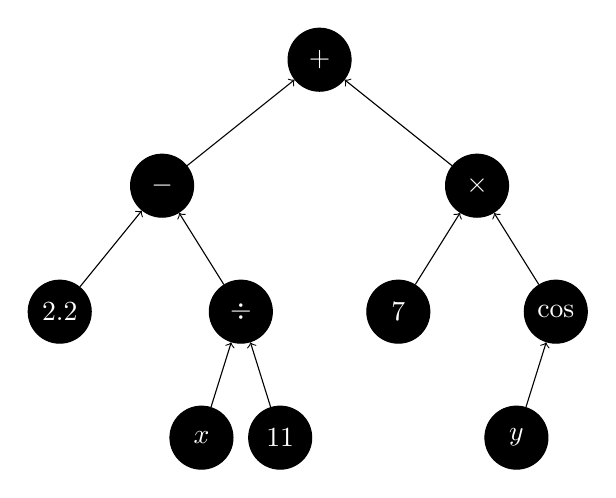
\begin{tikzpicture}[%
    node/.style = {circle, draw, minimum size = 0.8cm, align = flush center, inner sep = 0pt, fill = black, text = white},
    y = 0.8cm]

    \node[node] (x) at (5, 0) {$x$};
    \node[node] (11) at (6, 0) {$11$};
    \node[node] (y) at (9, 0) {$y$};
    \node[node] (div) at (5.5, 2) {$\div$};
    \node[node] (22) at (3.2, 2) {$2.2$};
    \node[node] (7) at (7.5, 2) {$7$};
    \node[node] (cos) at (9.5, 2) {$\cos$};
    \node[node] (sub) at (4.5, 4) {$-$};
    \node[node] (times) at (8.5, 4) {$\times$};
    \node[node] (plus) at (6.5, 6) {$+$};

    \draw[->] (x) -- (div);
    \draw[->] (11) -- (div);
    \draw[->] (y) -- (cos);
    \draw[->] (22) -- (sub);
    \draw[->] (div) -- (sub);
    \draw[->] (7) -- (times);
    \draw[->] (cos) -- (times);
    \draw[->] (sub) -- (plus);
    \draw[->] (times) -- (plus);
\end{tikzpicture}
}}
    \[
        \text{表达式: }\bigg(2.2 - \Big(\frac{x}{11}\Big)\bigg) + \big(7 \times \cos(y)\big)\text{.}
    \]
\end{minipage}
\end{frame}

\subsection{会话 Session}
\begin{frame}{\insertsection}{\insertsubsection}
233
\end{frame}